\documentclass[tikz]{standalone}
\usepackage{tikz}
\usetikzlibrary{arrows,automata}
\begin{document}
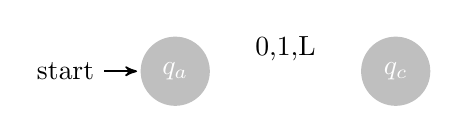
\begin{tikzpicture}[->,>=stealth',shorten >=1pt,auto,node distance=2.8cm,
                    semithick]
  \tikzstyle{every state}=[fill=lightgray,draw=none,text=white]

  \node[initial,state] (A) {$q_a$};
  \node[state] (C) [right of=A] {$q_c$};

  \path (A) -- node {0,1,L} (C);
\end{tikzpicture}
\end{document}